\documentclass[a4paper,12pt]{article}

\usepackage[T2A]{fontenc} 
\usepackage[utf8]{inputenc}
\usepackage[english,russian]{babel}
\usepackage{listings}
\usepackage[dvips]{graphicx}
\usepackage{indentfirst}
\usepackage{color}
\usepackage{hyperref}
\usepackage{amsmath}
\usepackage{amssymb}
\usepackage{geometry}
\geometry{left=1.5cm}
\geometry{right=1.5cm}
\geometry{top=1cm}
\geometry{bottom=2cm}

\graphicspath{{images/}}

\begin{document}
\sloppy

\lstset{
	basicstyle=\small,
	stringstyle=\ttfamily,
	showstringspaces=false,
	columns=fixed,
	breaklines=true,
	numbers=right,
	numberstyle=\tiny
}

\newtheorem{Def}{Определение}[section]
\newtheorem{Th}{Теорема}
\newtheorem{Lem}[Th]{Лемма}
\newenvironment{Proof}
	{\par\noindent{\bf Доказательство.}}
	{\hfill$\scriptstyle\blacksquare$}
\newenvironment{Solution}
	{\par\noindent{\bf Решение.}}
	{\hfill$\scriptstyle\blacksquare$}


\begin{flushright}
	Кринкин М. Ю. группа 504 (SE)
\end{flushright}

\section{Домашнее задание 8}

\paragraph{Задание 1.} Доказать, что число Каталана $c_n$ равно:
\begin{enumerate}
\item количеству способов разбиения выпуклого $(n+2)$ - уголтника на треугольники диагоналями, не пересекающимися внутри многоугольника;

\item количеству способов соединения $2n$ точек на окружности $n$ непересекающимися отрезками;

\item количеству монотонных отображений из $n$-множества $\left[n\right] = \{1, 2, ..., n\}$ в $\left[n\right]$, таких, что $f\left(i\right) \le i$ для любого $i \in \left[n\right]$;

\item количеству двоичных деревьев (из любой вершины выходит не более двух ребер) c $n$ вершинами;

\item количеству плоских деревьев с $\left(n+1\right)$ вершшинами;

\item количеству перестановок $a_1a_2...a_n$ множества $\left[n\right]$, которые можно упорядочить по возрастанию с помощью единственного стека.
\end{enumerate}

\begin{Solution}
Пронумеруем все вершины от $1$ до $n+2$. Каждый треугольник будет опираться на некоторую сторону $(i, i+1)$, более того на эту сторону будет опираться только один треугольник. Рассмотрим сторону $(n+1, n+2)$ количество способов добавить к стороне вершину, так чтобы получился треугольник равно количеству возможных вершин $n$ - штук.

\begin{figure}[h]
\center{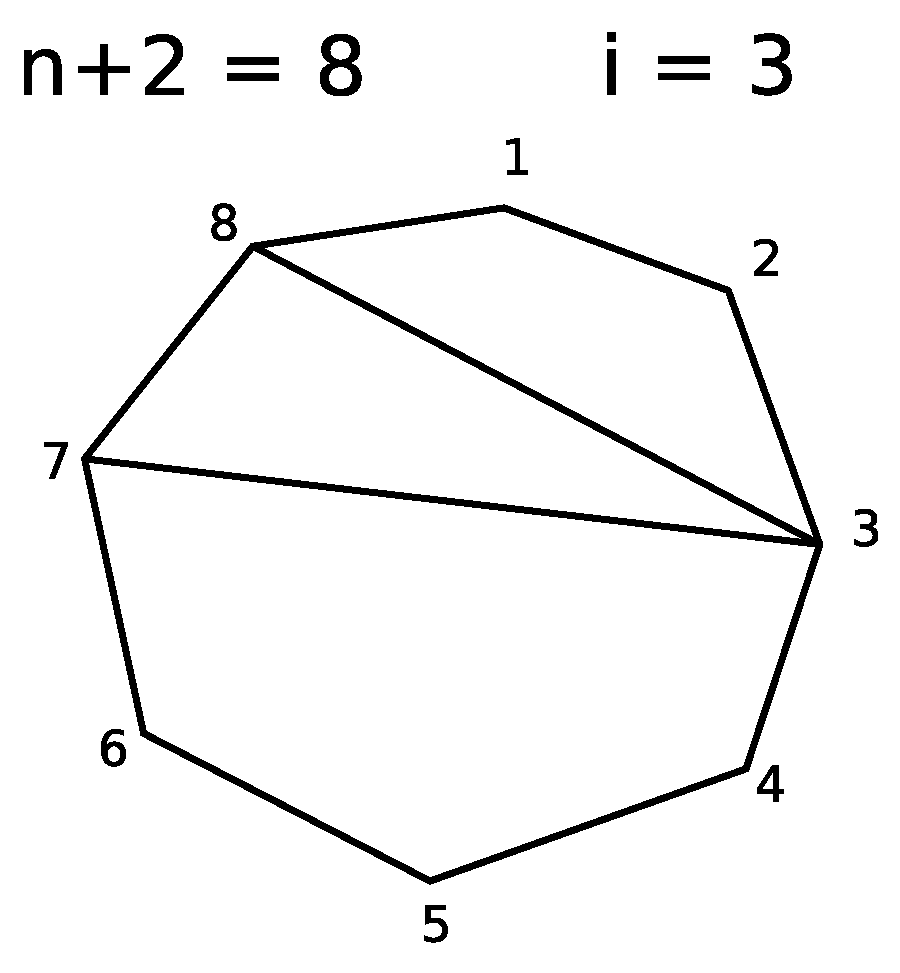
\includegraphics[width=0.3\linewidth]{simplex}}
\caption{Пример выбора опорной вершины и разбиения многоугольника}
\label{img::simplex}
\end{figure}

Пусть мы выбрали эту вершину и это вершина $i$ (см. рисунок \ref{img::simplex}). Тогда после <<вырезания>> треугольника получаем два многоугольника с количеством вершин $i+1$ и $n + 2 - i$ (т. е. вершина $i$ продублировалась в оба многоугольника, а $n+1$ и $n+2$ поделились между ними). Разбить первый из них можно $c_{i-1}$ способами, а второй $c_{n-i}$. Продолжаем процесс для каждого вновь образовонного многоугольника, пока не получим треугольник.

$i$ принимает значения от $1$ до $n$, число способов триангуляции для выбранной вершины $i$ равно $c_{i-1} c_{n-i}$, суммируем по всем $i$:
\[
	c_{n} = c_0 c_{n-1} + c_1 c_{n-2} + ... + c_{n-1} c_0
\]
теперь осталось проверить только начальные условия, которые очевидно выполняются.

Рассмотрим вторую задачу. Пусть у нас $2n$ точек расставлено на окружности. Выбрем в нем начальную вершину пусть она имеет номер $1$. Соединить эту вершину можно только так, чтобы слева и справа от проведенного ребра оставалось четное количество точек, таким образом можно соединить вершину $1$ только с вершинами $2i$, где $i \in \overline{1,n}$ (с вершиной имеющей четный номер). После проведения отрезка $(1, 2i)$ наша задача распадается на две подзадачи, решение, которых эквивалентно решению исходной задачи меньшей размерности. Справа от $(1, 2i)$ остается $2i - 2 = 2(i-1)$ точек, а слева $2n - 2i + 2 = 2(n-i+1)$. Таким образом, если для $2k$ точек решением является число $c_k$, то $c_n = \sum_{i=1}^n c_{i-1} c_{n-i+1} = \sum_{i=0}^{n-1} c_i c_{n-i}$. Остается проверить лишь начальные условия.

Можно показать, что эта задача эквивалентна задаче о скобочных последовательностях. Каждая вершина $i$ от 1 до $2n$ соответствует $i$-ой позиции в строке скобок, причем, если вершина соединена с вершиной меньшего номера, то она соответствует закрывающей скобке, иначе вершина соответствует открывающей скобке. Очевидно, что такие пары соответствуют правильным скобочным последовательностям, и каждой скобочной последовательности спосотавляется $2n$ точек соединенных $n$ отрезками.

Строим двудольный граф отображения. Вершины первой доли - элементы из проецируемого множества, а вершины второй доли - элементы множества, на которое происходит отображение. Вершина из первой доли связана ребром с вершиной из второй доли, если элемент соответствующий вершине первой доли переходит в элемент соответствующий вершине второй доли. Пример графов для оторбажения из $\left[3\right]$ в $\left[3\right]$ приведен на рисунке \ref{img::mapping}.

\begin{figure}[h]
\center{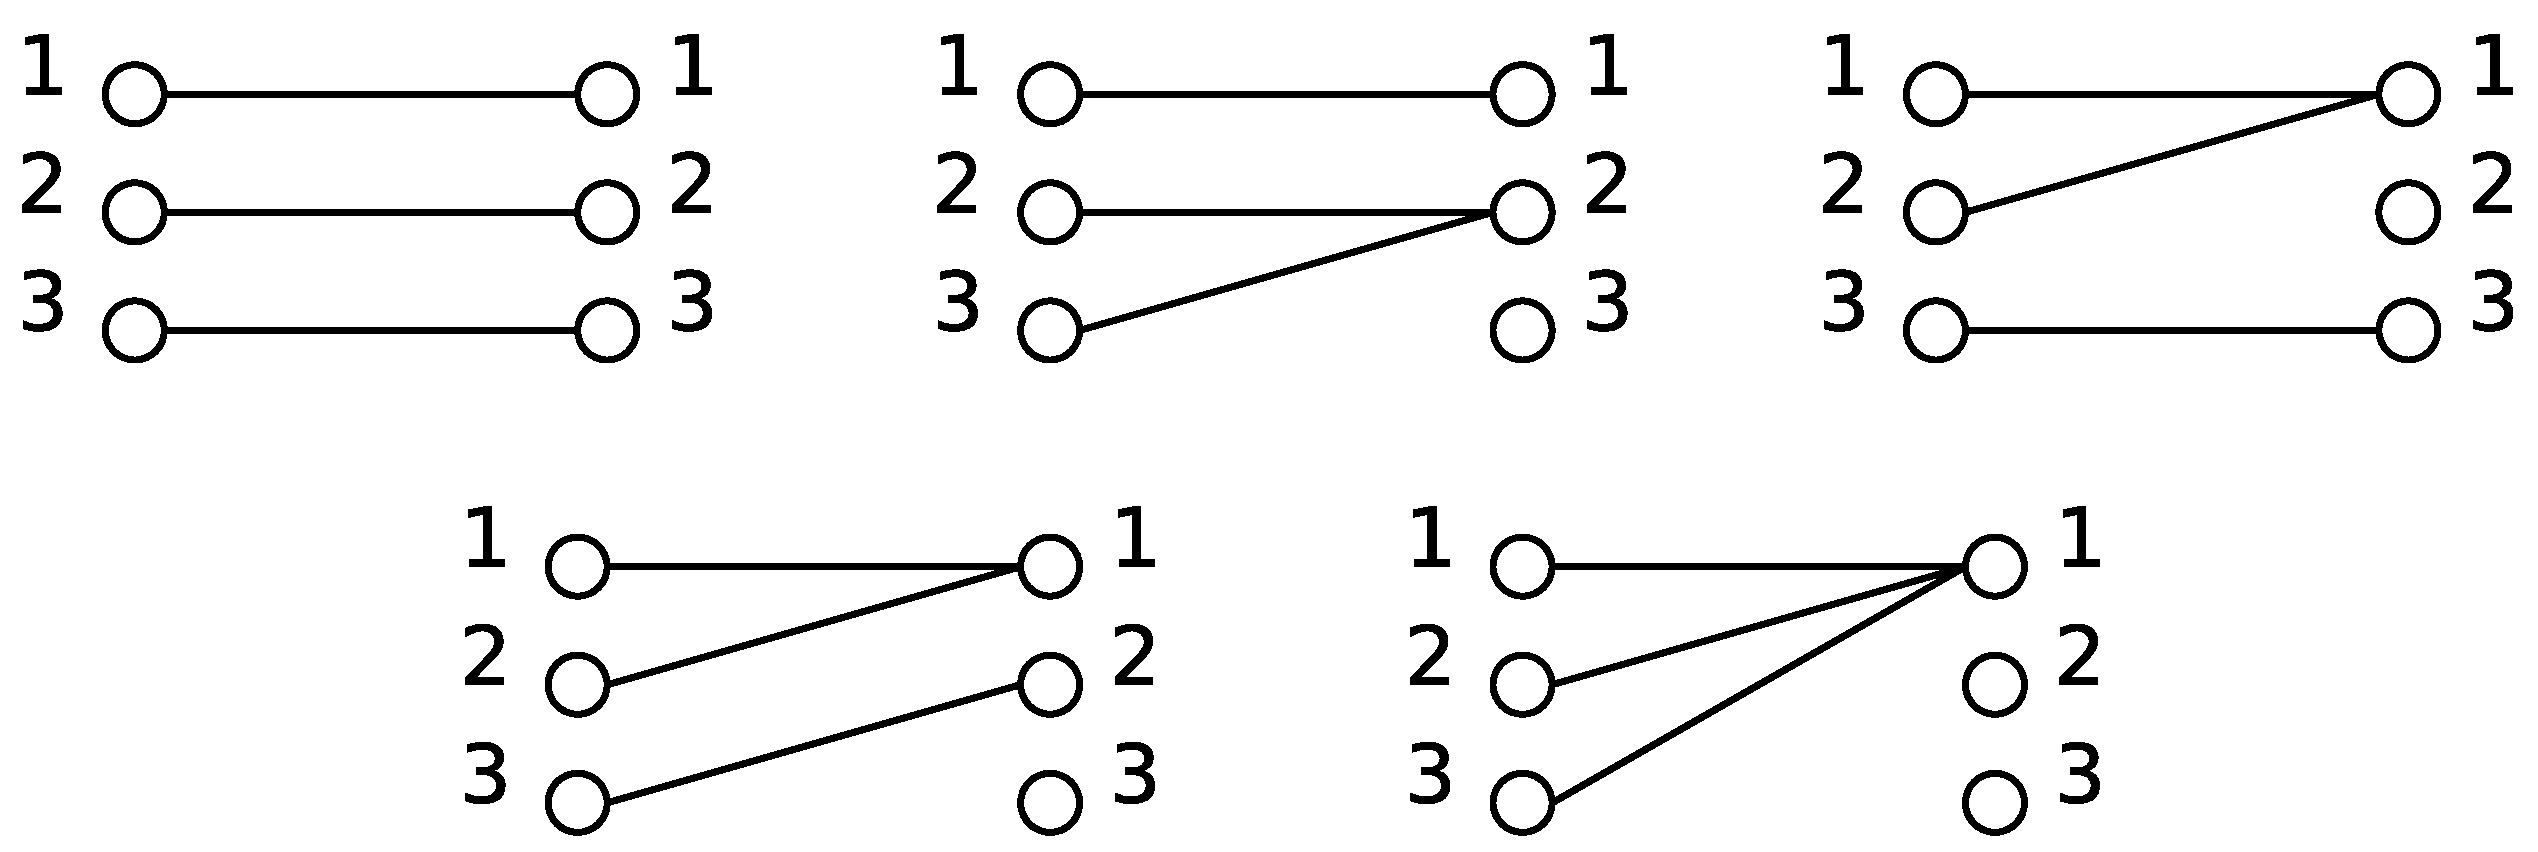
\includegraphics[width=0.5\linewidth]{mapping}}
\caption{Графы отображений}
\label{img::mapping}
\end{figure}

Каждому такому графу можно сопоставить путь на плоскости (см. рисунок \ref{img::paths}). На рисунке, на вертикали соответствующей $i$-ой вершине присутсвует стрелка вверх длины $k$, где $k$ - степень вершины $i$ из второй доли.

\begin{figure}[h]
\center{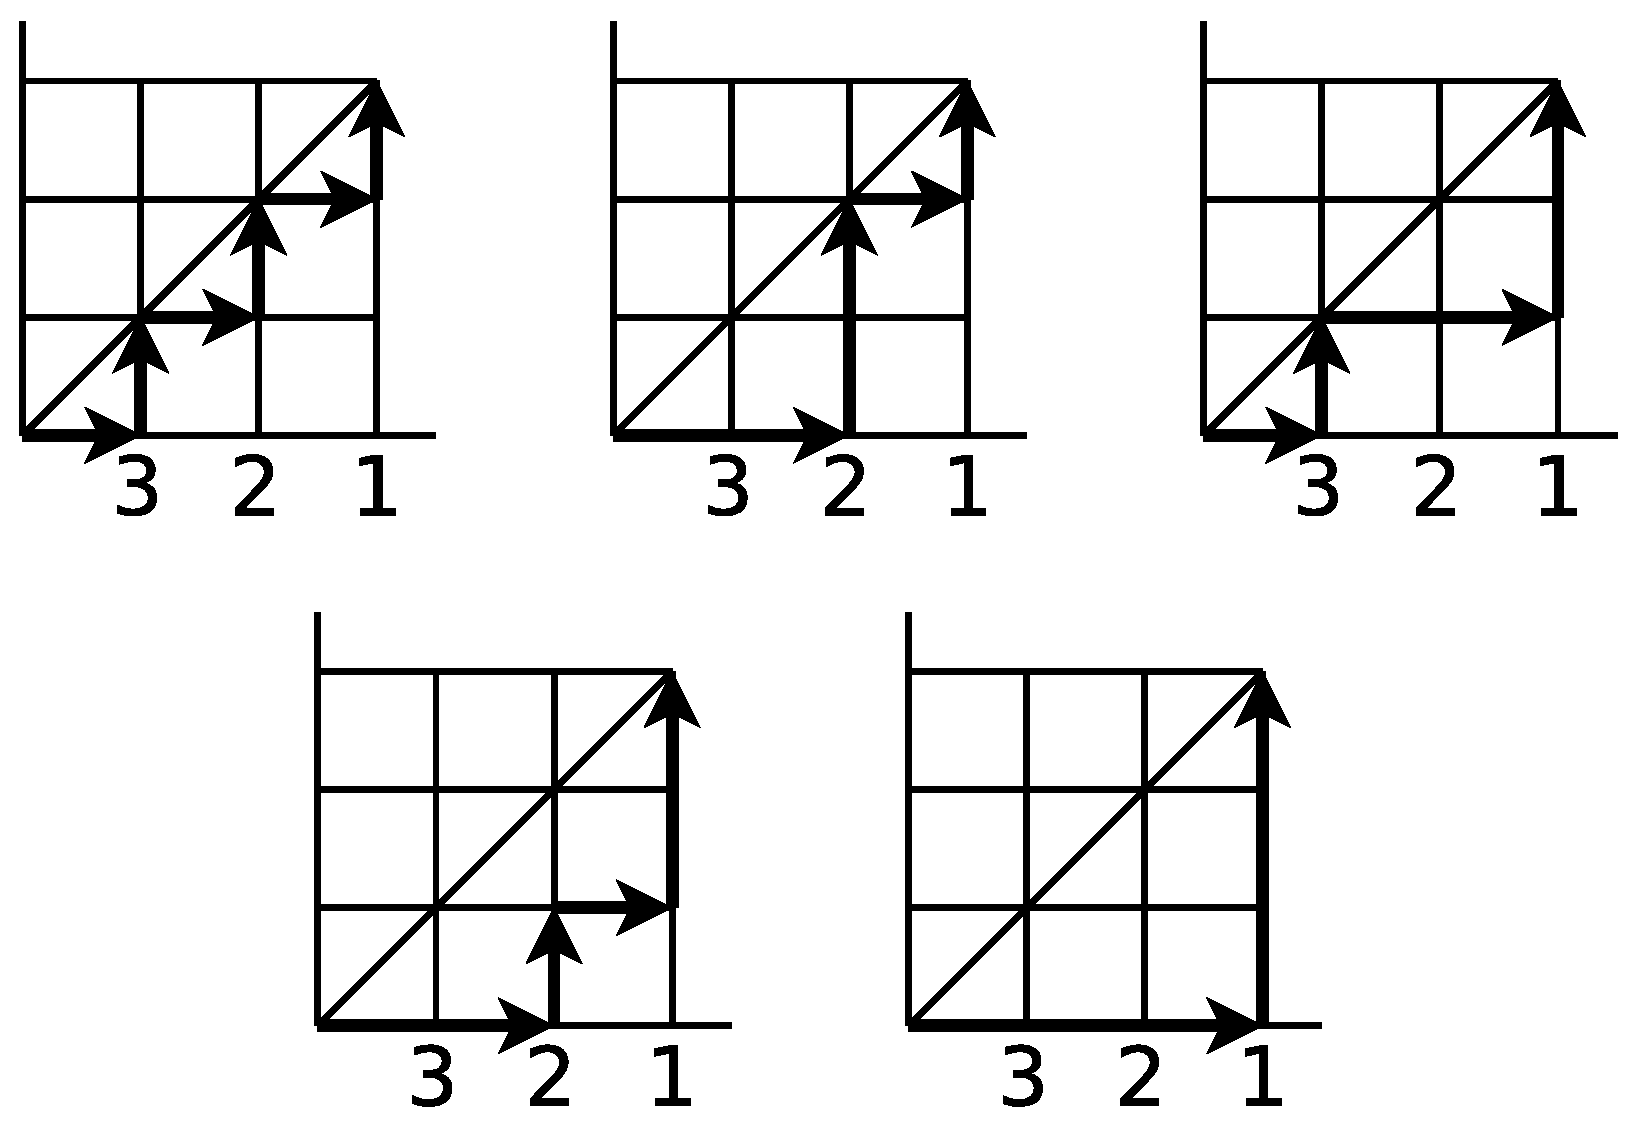
\includegraphics[width=0.5\linewidth]{paths}}
\caption{Пути на плоскости, соответствующие графам отображений}
\label{img::paths}
\end{figure}

Эти пути аналогичны путям Дика, и их количество также определяется числами Каталана. Но можно свести задачу и к задаче о скобочных последовательностях: шаг на единицу вправо - одна открывающая скобка, шаг на единицу вверх - закрывающая.

Четвертую пока пропустим.

В пятой задаче поступим следующим образом. Будем обходть дерево из некоторого корня пока не вернемся опять в корень. Если мы проходим по ребру нечетный раз (1, 3, 5 ...) то пишем открывающую скобку, иначе закрывающую. Таким образом получим, очевидно, только правильную скобочную последовательность.

В дереве $n-1$ ребер, пройти все ребра из некоторого корня и вернуться назад можно пройдя по каждому ребру ровно два раза, по такому обходу можно построить правильную скобочную последовательность из $2n$ скобок (по каждому ребру 2 раза).

Правда тут стоит заметить, что может существовать несколько таких обходов дерева, соответствующих разным скобочным последовательностям, но по каждой скобочной последовательности дерево восстанавливается однозначно, т. е. каждой скобочной последовательности мы можем сопоставить свое собственное дерево (если например восстанавливая дерево по скобочной последовательности нумеровать все ребра см. рис \ref{img::treetrav}).

Так как количество скобочных последовательностей определяется числами каталана, то и количество соответствующих им деревьев также определяется числами каталана. На рисунке \ref{img::treetrav} показано, как восстанавливать по скобочной последовательности дерево (и наоборот, как по дереву строить скобочную последовательность).

\begin{figure}[h]
\center{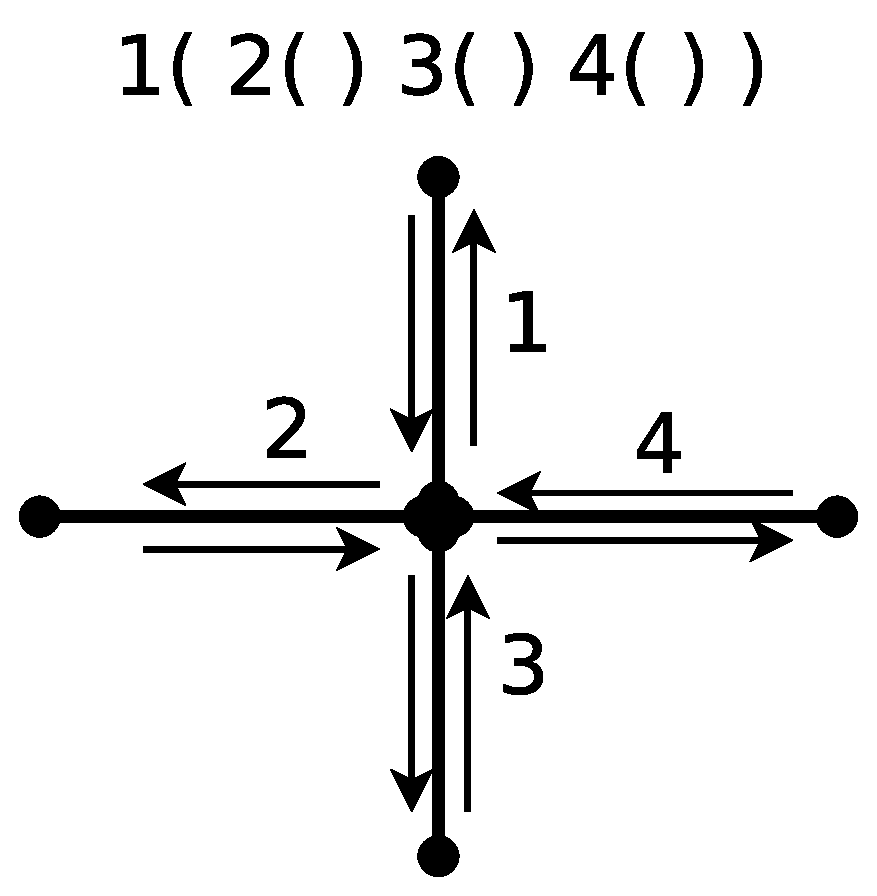
\includegraphics[width=0.3\linewidth]{treetrav}}
\caption{Соответствие деревьев и скобочных последовательностей}
\label{img::treetrav}
\end{figure}

\end{Solution}


\paragraph{Здание 2.} Числом Моцкина $M_n$ называется число решоточных путей из точки $(0,0)$ в точку $(0,n)$, не опускающихся ниже оси $y=0$ и составленных из шагов $(1,0)$, $(1,1)$ и $(1,-1)$. Найти для этих чисел рекуррентное соотношение и обыкновенную производящую функцию.

\begin{Solution}
Закодируем каждый путь Моцкина некоторым словом, вектору $\left(1,1\right)$ сопоставим открывающую скобку, вектору $\left(1,-1\right)$ сопоставим закрывающую скобку, а $\left(1, 0\right)$ - букву $x$. Если слово начинается с $x$, то <<отрезав>> $x$ опять получаем слово Моцкина, но длины на единицу меньше, если же начинается с открывающей скобки, то находим соответствующую закрывающую скобку, т. е. имеем $\left(s_1\right)s_2$, $s_1$ и $s_2$ - правильные слова Моцкина, и если $\left|\left(s_1\right)s_2\right| = n$ и $\left|s_1\right| = i$, то $\left|s_2\right| = n-2-i$. Тогда просуммировав по всем $i = \overline{0,n-2}$, получаем рекуррентное соотношение:
\[
	m_{n+2} = m_{n+1} = \sum_{i=0}^n m_{n-i} m_i
\]
Теперь получим обыкновенную производящую функцию, пусть:
\[
	f\left(x\right) = m_0 + m_1 x + m_2 x^2 + m_3 x^3 + ...
\]
Домножим рекуррентное соотношение на $x^{n+2}$ и просуммируем по всем $n$:
\[
	\begin{split}
		& \sum_{n=0}^{\infty}m_{n+2} x^{n+2} = x \sum_{n=0}^{\infty} m_{n+1} x^{n+1} + x^2 \sum_{n=0}^{\infty} x^n \left[\sum_{i=0}^{n} m_{n-i} m_i\right] \Rightarrow \\
		& \Rightarrow f\left(x\right) - m_0 - m_1 = x \left(f\left(x\right) - m_0\right) + x^2 \left(f\left(x\right)\right)^2 \Rightarrow \\
		& \Rightarrow x^2 \left(f\left(x\right)\right)^2 + f\left(x\right)\left(x - 1\right) + m_0 + m_1 - x m_0 = 0\Rightarrow \\
		& \Rightarrow x^2 \left(f\left(x\right)\right)^2 + f\left(x\right)\left(x - 1\right) + 2 - x = 0 \\
		& f\left(x\right) = \frac{\left(1-x\right) - \sqrt{\left(1-x\right)^2 - 4x^2\left(2-x\right)}}{2x^2}
	\end{split}
\]
\end{Solution}

\paragraph{Задание 3.} Треугольник Дика перечисляет пути в положительном квадранте плоскости, выходящие из начала координат и составленные из векторов $(1,1)$ и $(1,-1)$. Найти для жтих чисел рекуррентное соотношение и производящую функцию вида:
\[
	f\left(t,x\right) = \sum_{n=0}^{\infty} \sum_{k=0}^n a_{n,k} x^k \frac{t^n}{n!}
\]

\begin{Solution}
Рекуррентное соотношение для чисел в узлах треугольника Дика:
\[
	a_{n,k} = a_{n-1, k-1} + a_{n-1,k+1}
\]
т. е. значение в точке $a_{n,k}$ определяется значениями в точках слева выше и слева ниже от нее.
Начальные условия для рекуррентного соотношения:
\[
	\begin{split}
		& a_{n,n} = 1 \\
		& a_{n,k} = 0, k > n \\
		& a_{n,k} = 0, k < 0
	\end{split}
\]
Далее немного схитрим, преобразуем треугольник Дика к следующему виду:
\[
	\begin{matrix}
		n \backslash k  & 0 & 1 & 2 & 3 & 4 \\
		0 & 1 \\
		1 & 1 & 1 \\
		2 & 1 & 2 & 2 \\
		3 & 1 & 3 & 5 & 5 \\
		4 & 1 & 4 & 9 & 14 & 14 \\
	\end{matrix}
\]
В преобразованном треугольнике Дика рекуррентное соотношение принимает вид:
\[
	d_{n+1,k+1} = d_{n, k+1} + d_{n+1, k}
\]
(элемент $(n,k)$ - сумма эелементов сверху и слева, т. е. каждая строка - диагональ исходного треугольника Дика)
Найдем двумерную экспоненциаьную функцию:
\[
	\begin{split}
		& d_{n+1, k+1} x^{k+1} = d_{n, k+1} x^{k+1} + x d_{n+1, k} x^k \Rightarrow \\
		& \Rightarrow \sum_{k=0}^{\infty} d_{n+1, k+1} x^{k+1} = \sum_{k=0}^{\infty} d_{n, k+1} x^{k+1} + x \sum_{k=0}^{\infty} d_{n+1, x} x^k \Rightarrow \\
		& \Rightarrow d_{n+1} - d_{n+1, 0} = d_{n} - d_{n, 0} + x d_{n+1} \Rightarrow d_{n+1} \left(1 - x\right) = d_{n} \Rightarrow \\
		& \Rightarrow \left(1 - x\right) \sum_{t = 0}^{\infty} d_{n+1} \frac{t^{n+1}}{\left(n+1\right)!} = \sum_{n=0}^{\infty} d_{n} \frac{t^{n+1}}{\left(n+1\right)!} \Rightarrow \\
		& \Rightarrow \left(1 - x\right)f'\left(t,x\right) = f\left(t,x\right) \Rightarrow f\left(t,x\right) = e^{\frac{t}{1-x}}
	\end{split}
\]
\end{Solution}
\end{document}
